% XeLaTeX can use any Mac OS X font. See the setromanfont command below.
% Input to XeLaTeX is full Unicode, so Unicode characters can be typed directly into the source.

% The next lines tell TeXShop to typeset with xelatex, and to open and save the source with Unicode encoding.

%!TEX TS-program = xelatex
%!TEX encoding = UTF-8 Unicode

\documentclass[10pt]{article}
\usepackage{geometry}                % See geometry.pdf to learn the layout options. There are lots.
\geometry{letterpaper}                   % ... or a4paper or a5paper or ... 
%\geometry{landscape}                % Activate for for rotated page geometry
%\usepackage[parfill]{parskip}    % Activate to begin paragraphs with an empty line rather than an indent
\usepackage{graphicx}
\usepackage{amssymb}
%%%% Package
\usepackage{amsmath,amssymb,amsthm}
\usepackage[UTF8,noindent]{ctex}
\usepackage{tikz}
\usetikzlibrary{calc}
\usetikzlibrary{arrows,snakes,backgrounds,shapes,shadows}
\usetikzlibrary{matrix,fit,positioning,decorations.pathmorphing}
\usepackage{listings}
\lstset{
keywordstyle=\color{blue!70},
frame=single,
basicstyle=\ttfamily,
commentstyle=\small\color{red},
breakindent=0pt,
rulesepcolor=\color{red!20!green!20!blue!20},
rulecolor=\color{black},
tabsize=4,
numbersep=5pt,
breaklines=true,
%% backgroundcolor=\color{red!10},
showspaces=false,
showtabs=false,
extendedchars=false,
escapeinside=``,
frame=no,
}

%%%% New Commands
\newcommand{\blue}{\textcolor{blue}}
\newcommand{\red}{\textcolor{red}}
\newcommand{\purple}{\textcolor{electricpurple}}
\newcommand{\ds}{\displaystyle}
\newcommand{\cd}{\cdots}
\newcommand{\dd}{\ddots}
\newcommand{\vd}{\vdots}
\newcommand{\id}{\iddots}


% Will Robertson's fontspec.sty can be used to simplify font choices.
% To experiment, open /Applications/Font Book to examine the fonts provided on Mac OS X,
% and change "Hoefler Text" to any of these choices.

\usepackage{fontspec,xltxtra,xunicode}
\defaultfontfeatures{Mapping=tex-text}
\setromanfont[Mapping=tex-text]{Hoefler Text}
\setsansfont[Scale=MatchLowercase,Mapping=tex-text]{Gill Sans}
\setmonofont[Scale=MatchLowercase]{Andale Mono}

\begin{document}
\renewcommand{\proofname}{\textbf{证明}}
%%%% New Theorem
\newtheorem{li}{例}
\newtheorem{jielun}{结论}
\newtheorem{dingli}{定理}
\newtheorem{mingti}{{命题}} 
\newtheorem{yinli}{{引理}} 
\newtheorem{tuilun}{{推论}}
\newtheorem{dingyi}{{定义}} 
\newtheorem*{jie}{{解}}
\newtheorem*{zhengming}{{证明}}
\newtheorem{zhu}{{注}}
\newtheorem*{zhu*}{{注}}
\newtheorem{xingzhi}{{性质}}
\newtheorem{wenti}{{问题}}

\title{二叉树、树与森林}
\author{张晓平}
%\date{}                                           % Activate to display a given date or no date
\maketitle

\begin{dingyi}
森林是$n\ge0$棵不相交树的集合。
\end{dingyi}
\section{树转换为二叉树}
将树转换为二叉树的步骤:
\begin{itemize}
\item[1.]  \blue{加线:}在所有兄弟结点之间加一条连线。   \item[2.]  \blue{去线:}对树中每个结点,只保留它和第一个孩子结点的连线,删除它与其他孩子结点之间的连线。 
\item[3.]  \blue{层次调整:}以树的根结点为轴心,将整棵树顺时针旋转一定角度,使之结构层次分明。注意第一个孩子是二叉树结点的左孩子,其兄弟转换过来的孩子是其右孩子。
\end{itemize}
\begin{figure}[htbp]
\centering
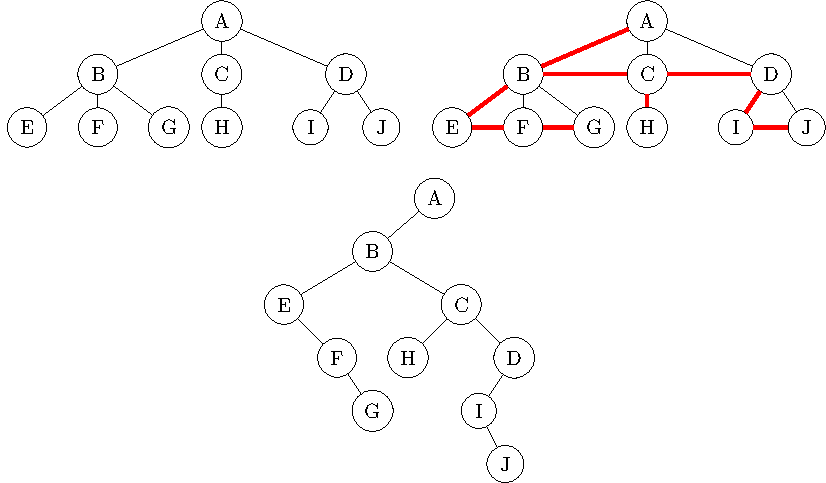
\includegraphics[width=5in]{TIKZ/forest/tree2btree.pdf}
\caption{树转换为二叉树}
\end{figure}


\section{森林转换为二叉树}
\begin{itemize}
\item[1.]  把每棵树转换为二叉树。 
\item[2.]  第一棵二叉树不动,从第二棵二叉树开始,依次把后一棵二叉树的根结点作为前一棵二叉树的根结点的右孩子,用线连接起来。当所有的二叉树连接起来后就得到了由森林转换来的二叉树。
\end{itemize}
\begin{figure}[htbp]
\centering
\begin{minipage}{0.45\textwidth}
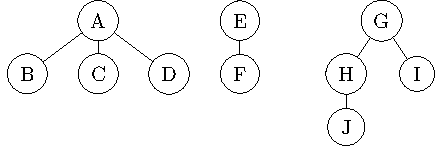
\includegraphics[width=2.4in]{TIKZ/forest/forest2btree1.pdf}  
\end{minipage}
\begin{minipage}{0.45\textwidth}
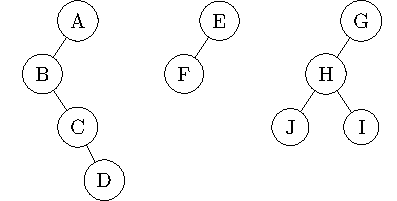
\includegraphics[width=2.4in]{TIKZ/forest/forest2btree2.pdf}  
\end{minipage}   
\begin{minipage}{0.45\textwidth}
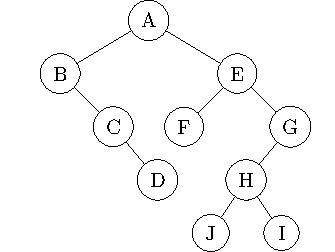
\includegraphics[width=2.in]{TIKZ/forest/forest2btree3.pdf}  
\end{minipage}
\caption{森林转换为二叉树} 
\end{figure}

\section{二叉树转换为树}
\begin{itemize}
\item[1.]  \blue{加线:}若某结点的左孩子存在,则将这个左孩子的右孩子、右孩子的右孩子、右孩子的右孩子的右孩子、$\cdots$,即左孩子的$n$个右孩子作为此结点的孩子。将该结点与这些右孩子用线连接起来。 
\item[2.]  \blue{去线:}删除原二叉树中所有结点与其右孩子的连线。
\item[3.]  \blue{层次调整:}使之结构层次分明。
\end{itemize}
\begin{figure}[htbp]
\centering
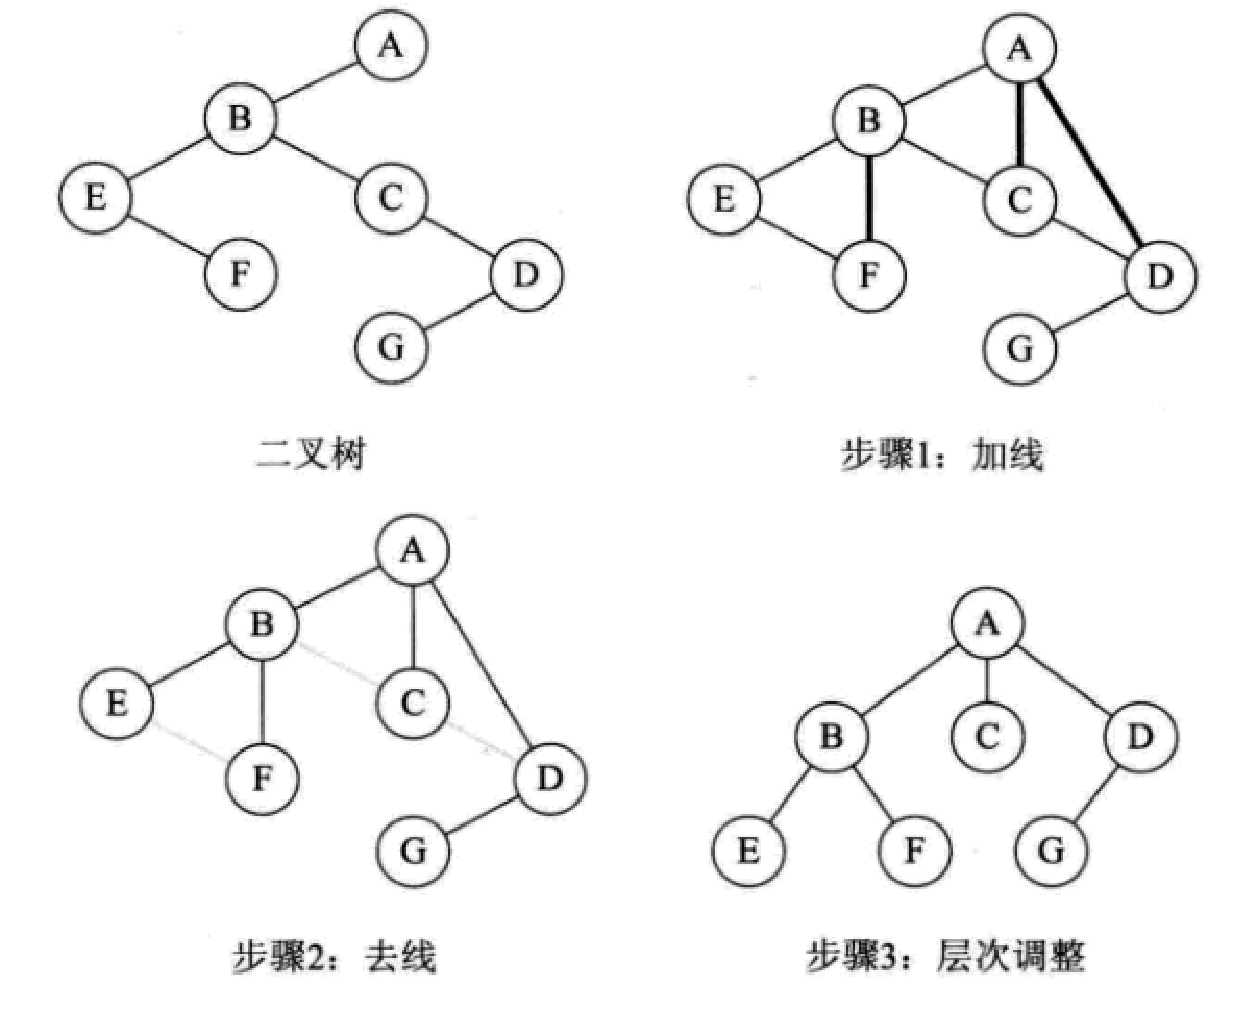
\includegraphics[width=4in]{fig/bitree2tree.pdf}
\caption{二叉树转换为树}
\end{figure}

\section{二叉树转换为森林}
判断一棵二叉树能够转换成一棵树还是森林,只要看这棵二叉树的根结点有没有右孩子,有就是森林,没有就是一棵树。转换成森林的步骤:
\begin{itemize}
\item[1.] 从根结点开始,若右孩子存在,则把与右孩子结点的连线删除,再查看分离后的二叉树,若右孩子存在,则连线删除,$\cdots$,直到所有右孩子连线都删除为止,得到分离的二叉树。 
\item[2.] 再将每棵分离后的二叉树转换为树即可。
\end{itemize}
\begin{figure}[htbp]
\centering
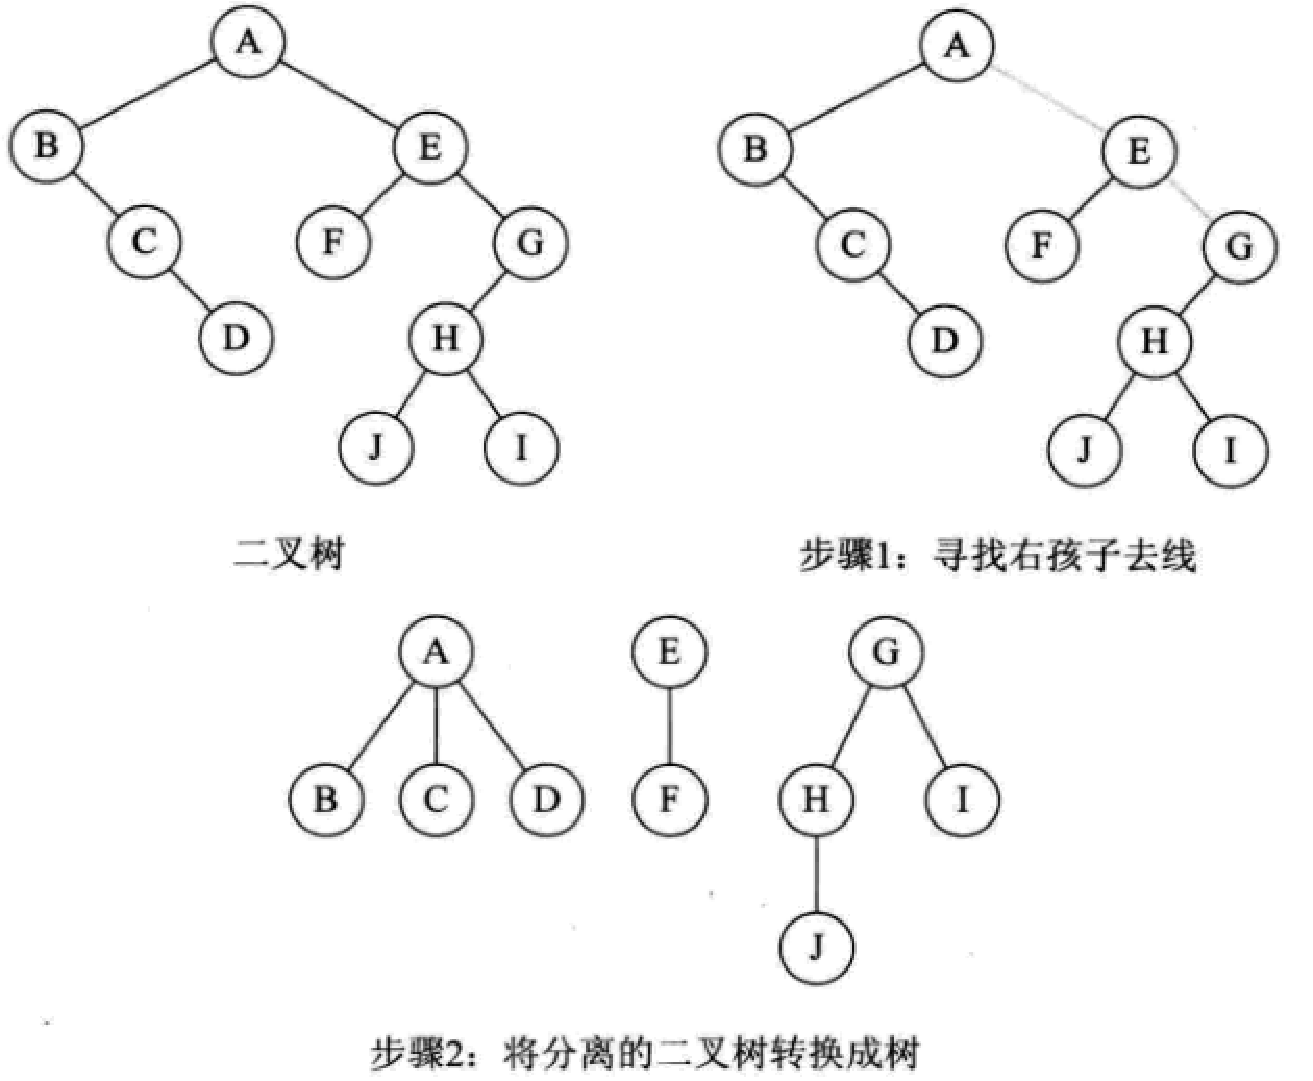
\includegraphics[width=4in]{fig/bitree2forest.pdf}
\caption{二叉树转换为森林}
\end{figure}

\section{树和森林的遍历}
\subsection{树的遍历}
树的遍历分为两种方式:
\begin{itemize}
\item[1.] \blue{先根遍历:}先访问树的根结点,然后依次先根遍历根的每棵子树。
\item[2.] \blue{后根遍历:}先依次后根遍历每棵子树,然后再访问根结点。
\end{itemize}

\begin{figure}[htbp]
\centering
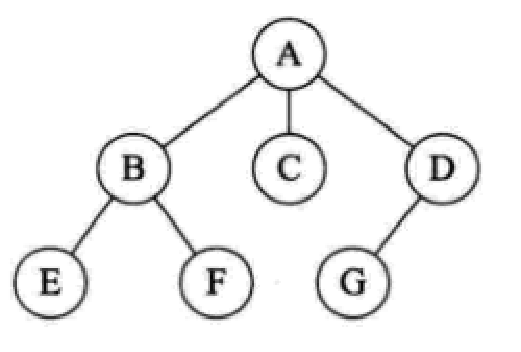
\includegraphics[width=1.8in]{fig/tree.pdf}
\caption{先根遍历序列为ABEFCDG; ~
后根遍历序列为EFBCGDA。}
\end{figure}

\subsection{森林的遍历}
记森林F转换而成的树为T。先序遍历森林F与先序遍历T自然对应;中序遍历森林F与中序遍历T自然对应。

先序遍历T等价于F的森林先序遍历,定义如下:
\begin{itemize}
\item[(1)] 若F为空,返回; 
\item[(2)] 访问F中的第一棵树的树根;
\item[(3)] 森林先序遍历F中第一棵树的所有子树;
\item[(3)] 森林先序遍历F中除第一棵树以外的所有子树。
\end{itemize} 

中序遍历T等价于F的森林中序遍历,定义如下:
\begin{itemize}
\item[(1)] 若F为空,返回; 
\item[(2)] 森林中序遍历F中第一棵树的所有子树;
\item[(3)] 访问F中的第一棵树的树根;
\item[(3)] 森林中序遍历F中除第一棵树以外的所有子树。
\end{itemize} 

\begin{figure}[htbp]
\centering
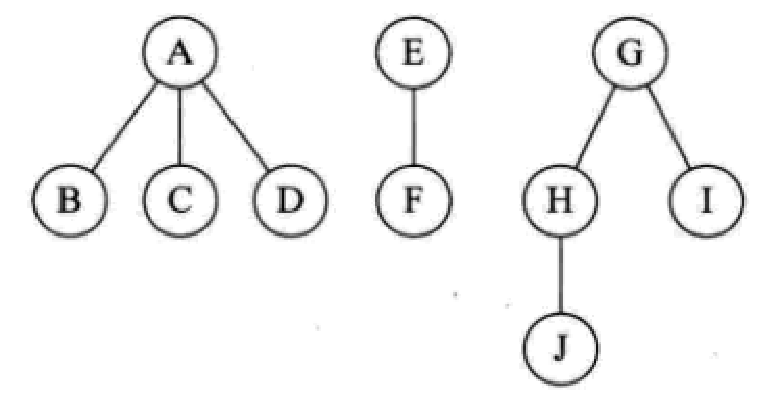
\includegraphics[width=2in]{fig/forest.pdf}
\caption{先序遍历序列为ABCDEFGHJI; ~
中序遍历序列为BCDAFEJHIG。}
\end{figure}

先序、中序遍历森林等价于先序、中序遍历对应的二叉树,而后序遍历森林与后序遍历对应的二叉树无自然对应。森林后序遍历定义如下:
\begin{itemize}
\item[(1)] 若F为空,返回; 
\item[(2)] 森林后序遍历F中第一棵树的所有子树;
\item[(3)] 森林后序遍历F中除第一棵树以外的所有子树;
\item[(3)] 访问F中的第一棵树的树根。
\end{itemize} 

%\begin{figure}[htbp]
%\centering
%\begin{minipage}{0.45\textwidth}
%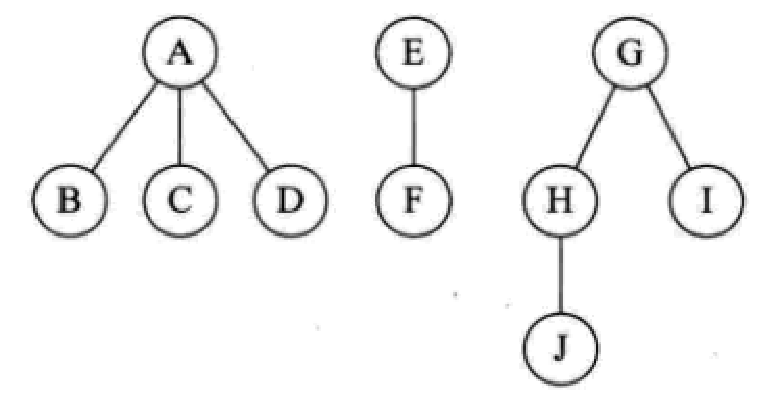
\includegraphics[width=2.2in]{fig/forest.pdf}  
%\end{minipage}
%\begin{minipage}{0.45\textwidth}
%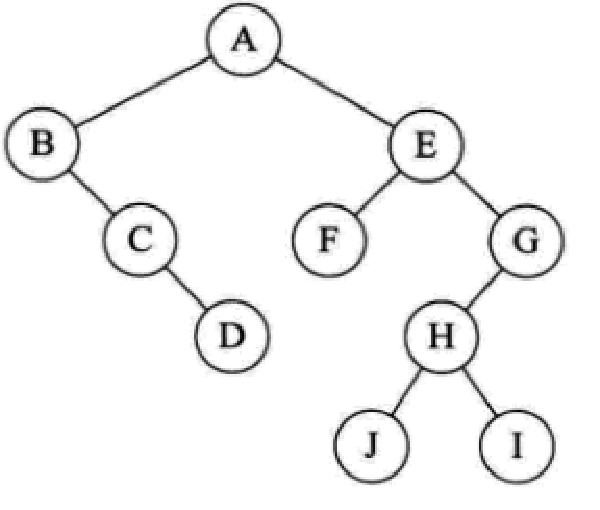
\includegraphics[width=1.6in]{fig/bitree.pdf}  
%\end{minipage}   
%\caption{森林的前序遍历和转换二叉树的前序遍历结果相同,森林的中序遍历和转换二叉树的中序遍历结果相同。} 
%\end{figure}


\end{document}  